\documentclass[10pt,conference,compsocconf]{IEEEtran}

%\usepackage{times}
%\usepackage{balance}
\usepackage{url}
\usepackage{graphicx}	% For figure environment
\usepackage[pdftex]{hyperref}
\usepackage[utf8]{inputenc} % To make umlauts and other symbols correct

\begin{document}
\title{Image restoration using dimensionality reduction in the Fourier domain}

\author{
  Patrick Bänziger, Kaspar Etter, Jan Rüegg \\
  Department of Computer Science, ETH Zurich, Switzerland
}

\maketitle

\begin{abstract}
  This paper suggests a novel approach to restore noisy images.
  ((( TODO )))
  The abstract should really be written last, along with the title of
the paper. The four points that should be covered~\cite{jones08}:
\begin{enumerate}
\item State the problem.
\item Say why it is an interesting problem.
\item Say what your solution achieves. (CLAIM!)
\item Say what follows from your solution.
\end{enumerate}
\end{abstract}

\section{Introduction}
In image inpainting, the aim is to restore an image from a disturbed source.
These disturbances may, for example, result from a transmission over a noisy channel or from a degraded physical copy of the original image. Another application is object removal where a part of the image to be removed and the hole to be filled using inpainting. (((EXPAND)))\\
Our approach focuses on the first inpainting application. We use an iterative algorithm with dimensionality reduction in the Fourier domain paired with several adaptations to improve speed and reduce artifacts in the output.
((( TODO )))\\

The aim of writing a paper is to infect the mind of your reader with
the brilliance of your idea \cite{jones08}. 
The hope is that after reading your
paper, the audience will be convinced to try out your idea. In other
words, it is the medium to transport the idea from your head to your
reader's head. 


\section{Methods}
\subsection{Related work}
((( TODO )))

\subsection{New approach}
(((REWRITE)))
We combine several ideas in our approach to obtain a inpainting algorithm that provides good results and fast performance.
Our algorithm requires as input the image which shall be restored and a mask which indicates the pixels that shall be filled. Such a mask can be created by the user or automatically (e.g. when a checksum algorithm detects faulty pixels).\\
The main inspiration behind our algorithm is that we try to interpolate the pixels from its neighboring values. By this we add some noise compared to the original, undamaged image. We then try to use dimensionality reduction to filter out this generated noise to reconstruct the image.\\

We use an iterative scheme to determine the right parameters used in our algorithm. For this, we use cross-validation: We randomly remove a percentage of pixels from the image as a validation set. (((STILL VALID?))) We then use this set to test the accuracy of our parameters and determine the best set of parameters for this image.

We then proceed to the main steps of the algorithm:
\begin{enumerate}
\label{algo}
\item \label{algo:step1}
We use a Gaussian to interpolate the missing pixels indicated by the mask, using a convolution operation. Both $\sigma$ and the size of the Gaussian matrix are determined by the cross-validation. (((TODO?!)))
This step is required by the Fourier transform which cannot ignore samples. (((Humm)))

\item \label{algo:step2}
We transform the image to the Fourier domain. In this domain we set the magnitudes of all frequencies to zero which are below the $n$-th percentile threshold. Again, our ideal cutoff $n$ is determined by cross-validation using a loop.

\item \label{algo:step3}
In this last step, we invert the Fourier transform and combine the reconstructed image with the undamaged part of the image, yielding our result.

\end{enumerate}

In our implementation, we use several tweaks to improve performance or quality:
\begin{itemize}
\item We perform the Fourier transform and thresholding on image patches to allow an individual threshold per patch.
\item To avoid discontinuity (Image \ref{fig:boundaryArtifacts}) at the boundary of the patches, we use a frame around the actual patch to capture more information. (Image \ref{fig:framing}) This frame is not filled in by the reconstructed patch from the Fourier step. The frames of adjacent patches are overlapping if the frame size is set to a value larger than zero. At the image boundaries, we replicate the outermost pixels to provide a sufficient frame.\end{itemize}
((( TODO )))
Describe your idea and how it was implemented to solve
  the problem. Survey the related work, giving credit where credit is
  due. 
  
  The style in this section should read as if you were verbally
describing the conduct of the experiment. 
The methods section is not a step-by-step, directive,
protocol as you might see in your lab manual, but detailed enough such
that an interested reader can reproduce your
work~\cite{anderson04,wavelab}.
The methods
section should describe what was
done to answer the research question, describe how it was done,
justify the experimental design, and
explain how the results were analyzed.

The methods section of a research paper provides the information by
which a study's validity is judged.
Therefore, it requires a clear and precise description of how an
experiment was done, and the rationale
for why specific experimental procedures were chosen.
It is usually helpful to
structure the methods section by~\cite{kallet04methods}:
\begin{enumerate}
\item Describing the algorithms used in the study, briefly including
  details such as hyperparameter values (e.g. thresholds), and
  preprocessing steps (e.g. normalizing the data to have mean value of
  zero).
\item Explaining how the materials were prepared, for example the
  images used and their resolution.
\item Describing the research protocol, for example which examples
  were used for estimating the parameters (training) and which were
  used for computing performance.
\item Explaining how measurements were made and what
  calculations were performed. Do not reproduce the full source code in
  the paper, but explain the key steps.
\end{enumerate}

\subsection{Online threshold estimation}
In the algorithm as described above, we have many different parameters that are required to be tuned

\subsection{Offline parameter estimation}


\section{Results}
We evaluated two versions of our algorithm: An iterative variant and a non-iterative variant.
Our iterative variant repeats 
 ((( TODO )))
 
 We compare our algorithm with the following two baseline algorithms:
 \begin{enumerate}
 \item A simple inpainting algorithm using (((TODO )))
 \item A matching pursuit algorithm with a dictionary consisting of (((TODO)))
 \end{enumerate}
 
 We tested our algorithm and the two baselines on a set of natural images and further on a set of artificially created ones. (((TODO More than 1))) 
 
 ((( TODO )))
  Show evidence to support your claims made in the
  introduction. 
  
Organize the results section based on the sequence of table and
figures you include. Prepare the tables and figures as soon as all
the data are analyzed and arrange them in the sequence that best
presents your findings in a logical way. A good strategy is to note,
on a draft of each table or figure, the one or two key results you
want to address in the text portion of the results.
The information from the figures is
summarized in Table~\ref{tab:fourier-wavelet}.

\begin{table*}[htbp]
  \centering
  \begin{tabular}[c]{|l||l|l|l|}
    \hline
    Basis&Support&Suitable signals&Unsuitable signals\\
    \hline
    Fourier&global&sine like&localized\\
    wavelet&local&localized&sine like\\
    \hline
  \end{tabular}
  \caption{Characteristics of Fourier and wavelet basis.}
  \label{tab:fourier-wavelet}
\end{table*}

When reporting computational or measurement results, always
report the mean (average value) along with a measure of variablility
(standard deviation(s) or standard error of the mean).

You compare your novel algorithm to \emph{at least two baseline
  algorithms}. For the baselines, you can use the implementations you
developed as part of the programming assignments.

\section{Discussion}
  Discuss the strengths and weaknesses of your
  approach, based on the results. Point out the implications of your  
  novel idea on the application concerned. (((( TODO ))))


\subsection{Figures and Tables}


\begin{figure}[tbp]
  \centering
  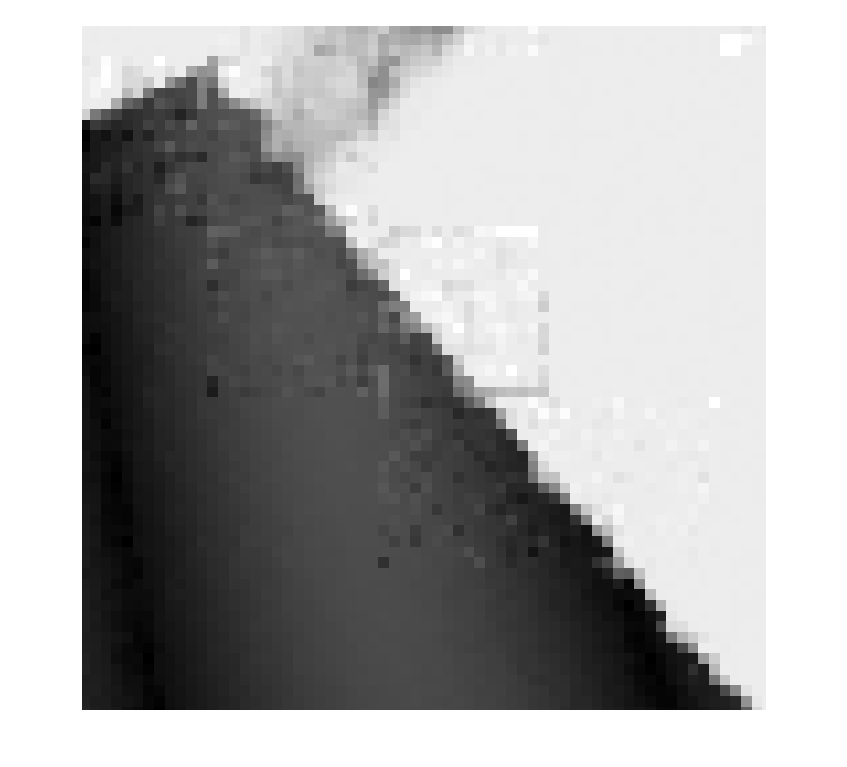
\includegraphics[width=\columnwidth]{images/boundaryArtifact_noframe}
  \caption{Artifacts that occur without a frame (frame size = 0). The patches are recognizable in the reconstruction}
  \label{fig:boundaryArtifacts}
\end{figure}

\begin{figure}[tbp]
  \centering
  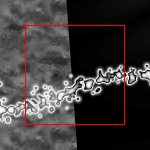
\includegraphics[width=\columnwidth]{images/imageFraming}
  \caption{Only the inner patch (marked red) is reconstructed in one step while the frame only provides additional signal. (Undistorted image shown) }
  \label{fig:framing}
\end{figure}

((( TODO: Plot missingPixel\% vs. accuracy (vs. speed?) )))

Use examples and illustrations to clarify ideas and results. For
example, by comparing Figure~\ref{fig:framing} and
Figure~\ref{fig:flowchart}, we can see the two different
situations where Fourier and wavelet basis perform well. 

\section{Summary}
(((( TODO ))))
  Summarise your contributions in light of the new
  results.
  

\section*{Acknowledgements}
We would like to recognize and thank the following individuals or groups for their contribution to this work:\\
Our implementation is based on the inpainting and evaluation framework provided by the course "Computer Intelligence Lab" held by Prof. Joachim Buhmann at ETH Zürich.
(((( TODO ))))


\bibliographystyle{IEEEtran}
\bibliography{biblio}

\clearpage
\section{Appendix}
\begin{figure}[htbp]
  \centering
  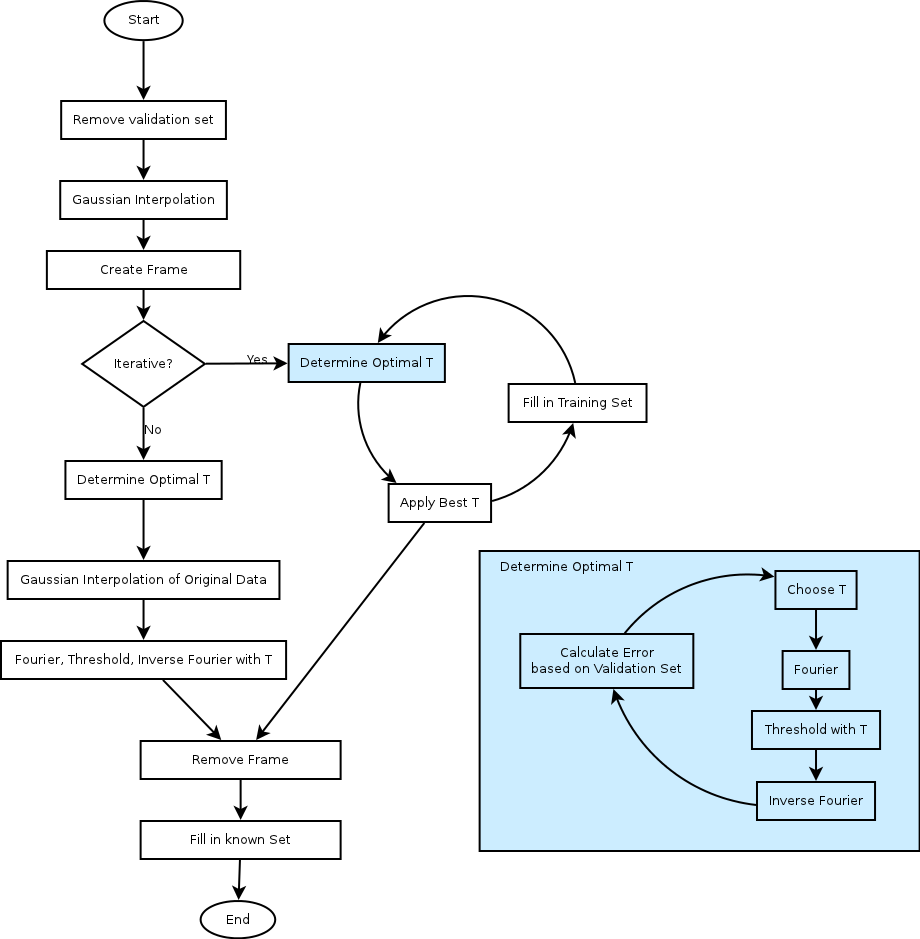
\includegraphics[width=\textwidth]{images/flowchart}
  \caption{The algorithm as a flow chart}
  \label{fig:flowchart}
\end{figure}
\end{document}
